% 1.2.1
\subsubsection{Thuật toán RSA }
\hspace*{2em} Thuật toán RSA (Rivest – Shamir – Adleman) là một trong những thuật toán mã hóa bất đối xứng phổ biến và có tính ứng dụng cao nhất hiện nay. RSA được phát triển vào năm 1977 bởi ba nhà khoa học Ronald Rivest, Adi Shamir và Leonard Adleman, dựa trên nguyên lý toán học của phép nhân và phân tích thừa số nguyên tố lớn.

\indent RSA hoạt động dựa trên hai khóa riêng biệt:
\begin{itemize}
  \item \textbf{Khóa công khai (Public Key):} dùng để mã hóa dữ liệu hoặc xác minh chữ ký số.

  \item \textbf{Khóa bí mật (Private Key):} dùng để giải mã dữ liệu hoặc tạo chữ ký số.
\end{itemize}

\indent Hình ~\ref{fig:cdm3} dưới đây mô tả quy trình mã hóa và giải mã trong thuật toán RSA, từ bước tạo khóa đến quá trình truyền và khôi phục dữ liệu.

\begin{figure}[H]
  \centering
  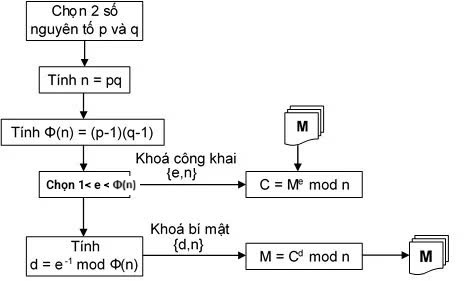
\includegraphics[width=.85\textwidth]{figures/pic3.png}
  \caption{Quy trình sinh khóa, mã hóa và giải mã trong thuật toán RSA.}
  \label{fig:cdm3}
\end{figure}

\indent Hình minh họa ba giai đoạn chính của RSA:
\begin{itemize}
  \item \textbf{Giai đoạn 1 – Sinh khóa:} Hai số nguyên tố lớn p và q được chọn để tính mô-đun n=p×q và giá trị Φ(n)=(p−1)(q−1). Sau đó chọn khóa công khai e và tính khóa bí mật d sao cho e×d≡1 mod  Φ(n).

  \item \textbf{Giai đoạn 2 – Mã hóa:}Thông điệp ban đầu M được mã hóa thành bản mã C=Me mod  n bằng khóa công khai.

  \item \textbf{Giai đoạn 3 – Giải mã:} Người nhận sử dụng khóa bí mật để giải mã M=Cd mod  n khôi phục lại nội dung ban đầu.
\end{itemize}

\indent Quy trình cho thấy độ an toàn của RSA đến từ việc khó phân tích mô-đun nnn để tìm ra hai số nguyên tố p và q, từ đó đảm bảo tính bảo mật và độ tin cậy của hệ thống mã hóa.
